\documentclass[12pt]{article}
\linespread{1}

% margins
\setlength{\textwidth}{6.5in}
\setlength{\textheight}{8.75in}
\setlength{\oddsidemargin}{-0.1in}
\setlength{\topmargin}{-0.1in}
\setlength{\baselineskip}{10pt}

% load packages
\usepackage{amsmath}
\usepackage{amsfonts}
\usepackage{lscape}
\usepackage[round]{natbib}
\usepackage{graphicx}
\graphicspath{{figures/}}
\usepackage{amssymb}
\usepackage{color}
\usepackage{hyperref}

% style setup
\bibliographystyle{plainnat}
\pagestyle{empty}
\setlength\parindent{0pt}
\setlength{\parskip}{\baselineskip}

% new commands
\newcommand{\indist}{\overset{d}{\rightarrow}}
\newcommand{\inprob}{\overset{P}{\rightarrow}}
\newcommand{\tabby}{\hspace{10pt}}
\newcommand{\ones}{{\bf 1}}
\newcommand{\tp}{\intercal}
\newcommand{\iprod}[2]{\langle #1 , #2 \rangle}

\newcommand{\note}[1]{\textcolor{red}{#1}}

% header
\title{HOSEA project notes}
\author{Peter MacDonald}
\date{\today}

\begin{document}

\maketitle

\section*{Data summary}

Data files on GreatLakes (SSH access with VPN) at path:
\begin{center}
  \texttt{../../nfs/turbo/umms-awaljee/umms-awaljee-HOSEA/Peter files}.
\end{center}

Contains .zip files basically corresponding to tables described in data dictionary
\begin{itemize}
  \item `alldxsX.zip' splits diagnoses into 3 tables? Due to file size constraints?
  \item What is `alldxscx.zip'?
  \item `colonoscopy',`EGDCPT',`EGDICD' also containsed in `procs.zip'.
  \item All Dxs are large files, about 1.5 GB, otherwise less than 1 GB except `labs\_cbc.zip'.
  \item CPT procedures and ICD procedures are combined into `procs.zip', which contains multiple files
\end{itemize}
Data dictionary (SAS summaries in Excel) here locally and on server.

Steps to open an interactive RStudio on GL:
\begin{enumerate}
  \item Activate UMich VPN
  \item Login at \url{greatlakes.arc-ts.umich.edu}
  \item Go to Interactive Apps, RStudio
  \item Fill information, note Slurm account = `\texttt{stats\_dept1}'
\end{enumerate}

Xuefei/Boang code imports data as a .csv, import .sas7bdat using \texttt{haven::read\_sas} (part of tidyverse). Should still work with .zip files.

{\bf 03/23:} Can read in zipped tables with interactive RStudio on GL. Permission denied to write new data to the folder (or even to create new subdirectories from terminal). Interactive RStudio will often crash if it has to run these large joins/filters, maybe develop things right now on a subset of the data and then move to the entire dataset later?

% \subsection*{Outline of tvc-project code}
%
% Fits a Cox PH model with time-varying covariates. \texttt{survival} package has some useful functions (\texttt{tvc}) for creating these covariates. Example code runs on sample data with random uniform placeholder values.

\section*{Data processing}

\begin{itemize}
  \item For a reference date (should be before the index date) $D$, want to predict if cancer occurs in the date window $[D,D+L]$ after a given time point, using clinical data from dates $[D-K,D]$. $L$ prediction window, $K$ collection window. \note{For this project, we will always have $L=1$ year, $K=2$ years. May need some sensitivity analysis down the road.}
  \item Some variables are `static' i.e. demographics, some are only observed once. Some (e.g. blood work) are observed, possibly multiple times at given `lab dates'.
  \item Q: static variables are collected at the index date, not the (theoretical) prediction date?
  \item Single events would just lead to one observation, if a patient gets several blood tests, could use say mean,max,min or mean,variance
  \item prior GI diagnoses,colonoscopies (events with no 'value') would be either yes/no or counts (How many prior GI diagnoses? Or keep each kind separate?), or is it valuable to keep time information as well (How long since the last GI diagnosis)
  \item Meds will need to be treated separately as well, novel covariates to construct here?
\end{itemize}

{\bf Storing `no value' lab events:} Include variables for {\em number of X} (in the prediction window) and {\em days since last X}.

Tables that can be processed this way: colonoscopy, EGDCPT, EDGICD, FOBT, GI procedures (CPT), GI procedures (ICD).

Tables like this that also have ICD code information are alldxs and priorgidxs, \note{ignore for now until we settle on a way of handling ICD information.}

Some cases with FOBT on back-to-back days? Are these actually different visits or just noise/processing times?

What if we treated {\em number of X} as the longitudinal predictor which increments by one at each event and apply the same summary procedure. Then max will be the count, min will be 0 for all, max/min slope will be useful if there are > 1 events, mean/total variation will be redundant as well. Can also treat 0/1 diagnosis events this way; make sure time since {\em X} is encoded.

$2 \times 6 = 12$ predictors

\note{How much redundancy is there in these tables, i.e. are EGDs also counted under GI procedures?}

{\bf Storing `valued' lab events:} Include variables for mean,max,min and variance of lab results (in the prediction window).

Weijing's paper (saved in HOSEA folder) uses 5 summaries for each numeric lab event: max, min, max slope, min slope, and total variation (mean of absolute value of slopes). All over the entire prediction window.

Tables that can be processed this way: Labs a1c, Labs BMP, Labs CBC, Labs CRP, Labs LFT, Labs lipid (33 total numeric values).

$6 \times (1 + 8 + 15 + 1 + 4 + 4) = 198$ predictors

{\bf Storing `static' variables:} These are the demographic variables in sample which are only measured once at the index date: race, height, weight, BMI, age, GERD, agent orange, smoking status, and Charlson score inputs (~ 18).

$18 + 8 = 26$ predictors

Smoking status is given in more detail in the SmokeHF table \note{Ignore this for now}.

{\bf Storing medication variables:} For each of the 2 drug types (H2R, PPI split by row into sub-tables), include an integrated intake over the 2 year window (based on dd and newenddate), and a max daily dose based on dd. \note{dd and newenddate are pre-cleaned by Jenny.}

$4 \times 2 = 8$ predictors

Approximate total right now is 182 predictors.

{\bf 03/30:} Read in all the SAS tables and save them as .rds files. Inspect tables and ask more questions, try and categorize variables.

{\bf 04/06:} Some zip files were too large to unzip directly in R? In particular alldxsX, labs\_cbc, labs\_bmp. Can unzip them with unzip terminal command.

Note the alldxsX tables are very large, 12-16GB each unzipped.

Also need to process main sample, impute missing values (with median, function from Xuefei/Boang code)

For subsample, read in a simple valued table (labs\_crp), and a unvalued/event table (labs\_fobt). Generalize code to read in other tables.

basic logistic regression stuff: sample a test set, fit on training, get train and test errors. Logistic regression generalizes well ($p << n$), gets about 77\% correct on the balanced subsample.

\subsection*{allmeds table}

Almost all the prescriptions have drug type either GA301 (14M rows) or GA900 (39M rows). About 50K missing and less than 1000 for other categories.

Med\_type seem to be the reliable indicator of the two types (H2R and PPI).

PPI: proton pump inhibitors (6 available active ingredients)

H2RA: H2 (histamine type-2) receptor antagonists (4+ available active ingredients)

\subsection*{Detailed missingness tables by blood lab type}

\note{Using old data, out of date as of August 20.}

\begin{center}
\begin{tabular}{|l|l|l|l|}
\hline
\textbf{A1C Labs} & Non-missing & Missing & Prop. missing \\ \hline
Controls & 3,283,993 & 3,353,720 & 0.51 \\ \hline
Cases & 5,462 & 5,933 & 0.52 \\ \hline
\end{tabular}
\end{center}

\begin{center}
\begin{tabular}{|l|l|l|l|}
\hline
\textbf{BMP Labs} & Non-missing & Missing & Prop. missing \\ \hline
Controls & 5,509,789 & 1,127,924 & 0.17 \\ \hline
Cases & 8,031 & 3,364 & 0.30 \\ \hline
\end{tabular}
\end{center}

\begin{center}
\begin{tabular}{|l|l|l|l|}
\hline
\textbf{CBC Labs} & Non-missing & Missing & Prop. missing \\ \hline
Controls & 5,327,609 & 1,310,104 & 0.20 \\ \hline
Cases & 5,812 & 5,583 & 0.49 \\ \hline
\end{tabular}
\end{center}

\begin{center}
\begin{tabular}{|l|l|l|l|}
\hline
\textbf{CRP Labs} & Non-missing & Missing & Prop. missing \\ \hline
Controls & 309,897 & 6,327,816 & 0.95 \\ \hline
Cases & 677 & 10,718 & 0.94 \\ \hline
\end{tabular}
\end{center}

\begin{center}
\begin{tabular}{|l|l|l|l|}
\hline
\textbf{LFT Labs} & Non-missing & Missing & Prop. missing \\ \hline
Controls & 5,127,835 & 1,509,878 & 0.23 \\ \hline
Cases & 6,044 & 5,351 & 0.47 \\ \hline
\end{tabular}
\end{center}

\begin{center}
\begin{tabular}{|l|l|l|l|}
\hline
\textbf{Lipid Labs} & Non-missing & Missing & Prop. missing \\ \hline
Controls & 5,377,320 & 1,260,393 & 0.19 \\ \hline
Cases & 7,728 & 3,667 & 0.32 \\ \hline
\end{tabular}
\end{center}

Summary table:
\begin{center}
\begin{tabular}{|l|l|l|}
\hline
\textbf{Prop. missing} & Controls & Cases \\ \hline
A1C Labs & 0.51 & 0.52 \\ \hline
BMP Labs & 0.17 & 0.30 \\ \hline
CBC Labs & 0.20 & 0.49 \\ \hline
CRP Labs & 0.95 & 0.94 \\ \hline
LFT Labs & 0.23 & 0.47 \\ \hline
A1C Labs & 0.19 & 0.32 \\ \hline
\end{tabular}
\end{center}

\subsection*{Detailed BMI vs Case comparison}

\note{Using old data, out of date as of June; updated numbers in the June 22 update.}

Counts:
\begin{center}
\begin{tabular}{|l|l|l|l|l|l|l|}
\hline
 \textbf{BMI} & $< 20$ & $\in (20,25]$ & $\in (25,30]$ & $\in (30,35]$ & $\in (35,40]$ & $> 40$  \\ \hline
Controls & 197,189 & 1,292,100 & 2,366,261 & 1,538,348 & 615,798 & 307,706 \\ \hline
Cases & 800 & 2,842 & 3,672 & 2,246 & 890 & 434 \\ \hline
\end{tabular}
\end{center}

Conditional probabilities:
\begin{center}
\begin{tabular}{|l|l|l|l|l|l|l|}
\hline
 \textbf{BMI} & $< 20$ & $\in (20,25]$ & $\in (25,30]$ & $\in (30,35]$ & $\in (35,40]$ & $> 40$  \\ \hline
$\mathbb{P}(Control | BMI)$ & 0.9960 & 0.9978 & 0.9985 & 0.9985 & 0.9986 & 0.9986 \\ \hline
$\mathbb{P}(Case | BMI)$ & 0.0040 & 0.0022 & 0.0015 & 0.0015 & 0.0014 & 0.0014 \\ \hline
\end{tabular}
\end{center}

\section*{Gitlab repo}

terminal code to access repo from login node:

\begin{verbatim}
  ../../nfs/turbo/umms-awaljee/umms-awaljee-HOSEA/Peter\ files/R_code/hosea-project
\end{verbatim}

\note{old\_code folder contains R code written before Gitlab was set up.}

Code is now stored in a Gitlab repo, locally at HOSEA/gitlab/hosea-project, and on GreatLakes as ...Peter files/R\_code/hosea-project. Ji can provide access to the account via Jessica Baker at the medical school.

Workflow: majority of development locally, push to Gitlab (terminal), pull on GreatLakes (terminal) and run in interactive RStudio session. Write filepaths relative to the 'Peter files' folder on GreatLakes.

Personal access token:
\begin{verbatim}
  46zuHm1buhzbG1XQ4oXp
\end{verbatim}

{\bf File structure:}
Processing in R begins with data saved as .sas7bdat files, after unzipping on terminal.
\begin{itemize}
  \item setup.R sets wd and loads packages
  \item utils.R defines small helper functions
  \item utils\_xgb.R defines helper functions for xgboost models and evaluation (data preparation, PDPs, AUCs, ...)
  \item utils\_missingcharl.R defines helper functions for coding new disease indicators (translated from Jenny's SQL code), and imputing missing values.
  \item sas\_to\_rds.R converts SAS database files to rds, performs reordering.
  \item master.R creates master table with start/end dates for prediction window
  \item process\_[...].R processes raw tables (.rds files) into longitudinal summaries by ID, processed version have '\_summary' appended to .rds file name.
  \item process\_new\_charlson.R processes filtered diagnosis tables into new disease indicators.
  \item link\_summaries.R combines all the summary tables and creates a single table complete\_data\_raw.rds
  \item link\_charlson.R combines all the charlson indicators tables and creates a raw and an imputed version.
  \item subsample.R takes a balanced subsample for testing (stores in R\_data/subsample)
  \item subsample\_cc.R finds a (mostly) complete cases/controls with no missing values, sample imputes and saves a complete test set.
  \item impute\_missing.R takes a table of the format of complete\_data\_raw.rds, prepares the tables, imputes with random sampling and/or chained regression models. impute\_models.R and impute\_multisamp.R contain helper functions.
  \item fit\_missing.R fits xgboost and logistic regression models \note{on the balanced subsample of 10,000} for different imputation approaches. Saves imputed datasets for training, test and validation (sub\_complete\_data\_impute.RData)
  \item fit\_varsubsets.R imports random sample imputed \note{balanced subsample} and fits models to different groups of variables (to assess information available in different groups)
  \item n\_visits.R creates a variable for number of visits (unique dates with an ICD code in the 4-year prediction window).
  \item n\_visits\_analysis.R does some additional analysis on this new variable, in relation to missingness of Charlson score inputs.
\end{itemize}

{\bf Saved data:}
\begin{itemize}
  \item Most data corresponds to an initial SAS table, or a processed/summarized version (with '\_summary') appended.
  \item alldxsX\_filter.rds for X from 1 to 5 has the alldxs records restricted to the current [index - 5y, index - 1y] prediction window. X = 'cx' corresponds to diagnoses for cases only
  \item master.rds contains IDs and start/end prediction dates
  \item complete\_data\_raw.rds fully linked table produced by link\_summaries.R
  \item cc\_complete\_data.rds contains a subset of records which are (mostly) non-missing (see subsample\_cc.R).
  \item n\_visits.rds contains a number of visits variable for all controls.
  \item n\_visits\_case.rds contains a number of visits variable for all cases.
  \item charlson\_[xxx].rds contains newly processed indicators for each of the component diseases, and GERD.
  \item charlson\_complete\_raw.rds contains the newly processed indicators in one table, with no imputation. Also includes number of visits.
  \item charlson\_complete\_impute.rds contains the newly processed indicators in one table, with zeros imputed according to the simple `geometric' model described below, based on number of visits. Also includes number of visits.
  \item {\bf Within 'subsample':}
  \begin{itemize}
    \item sub\_master.rds contains IDs and start/end prediction dates for the subsample
    \item sub\_complete\_data\_raw.rds subsets the complete data to the balanced subsample of 5000 cases and 5000 controls
    \item sub\_complete\_data\_impute.RData contains training test and validation subsets after applying different imputation methods (none, sample, median, regression)
  \end{itemize}
  \item {\bf Within 'models'}:
  \begin{itemize}
    \item multisamp\_models.RData contains the multiple random sample xgboost models created by fit\_missing.R
  \end{itemize}
\end{itemize}

\section*{Imputation}

Several methods are coded for variable imputation and comparison on the balanced subsample (see updates file).

\begin{itemize}
  \item {\bf Separate class} treats missing values as a categorical value for each predictor, and grows trees accordingly (with NAs sent down the optimal branch of each tree)
  \item {\bf Median} imputes all variables with their median; categorical variables with the most common class
  \item {\bf Regression} uses chained regressions to estimate missing values from observed values. Variables are transformed to z-scores, prediction is done on the z-scale, then transformed back to match the original distribution of observed values. 'Hybrid regression' implies that only the mean of each lab variable is imputed, then the remaining summaries (max,min,...) are selected jointly from observed values based on the nearest neighbor of the imputed mean.
  \item {\bf Single random sample} means that the variables are imputed at random from the observed values. Similar to hybrid regression, the longitudinal summaries of each blood lab variable are sampled jointly.
  \item {\bf Multiple random sample} means that the variables are imputed many times, and the xgboost model is grown progressively on each imputation of the data. As above the longitudinal summaries of each blood lab variable are sampled jointly. In this case the test set is also imputed many times, and preditions are averaged.
\end{itemize}

Rates of missingness are different between cases and controls, in general cases have more missing values. This is true for blood lab variables and for Charlson diagnosis codes.

\subsection*{Missingness of Charlson scores}

For each input to the Charlson score, patients are coded with a 1 if they received a particular Charlson code in the window of observation, a 0 if they received any Charlson code, but not that one, and NA if they received no codes. Hence the NA class contains people who have no data/not enough visits, but also people who have 0's across the board for all Charlson codes.

Currently, all NA's are treated as missing, and imputed to match the observed distribution of 1's and 0's.

A 'number of visits' variable may allow us to more intelligently impute these values (i.e. NA + lots of visits are more likely to a be a 0).

This can be determined by looking at the number of unique dates (after start and before end) in the ``alldxsX'' tables (in /unzipped\_data).

09/13: number of visits variable is now calculated, saved.

Suppose the following simple model for disease code missingness (for simplicity say there is a single diagnosis code), $Y_i$ denotes the true disease status, $O_i$ denotes whether the node is observed, and $V_i$ is the number of visits (opportunities to be coded). Assume $Y_i$ is independent of $V_i$ and work conditional on $V_i$.

We either observe $Y_{i,obs} = 1$ which means $Y_i=1$ and $O_i=1$, or $Y_{i,obs} = 0$ in any other case (in the data this groups the 0's and NA's interchangeably).

Let $p$ denote the true prevalence of disease (could model with two different prevalences, $p_{\mathrm{control}}$ and $p_{\mathrm{case}}$). The simple model assumes that at each visit, a patient with the disease has an independent chance to be coded for it with probability $\phi$. Then
\[
\mathbb{P}(Y_{i,obs}=1 | V_i) = p \cdot \mathbb{P}(\operatorname{Geom}(\phi) < V_i).
\]
This model can be used to estimate $\hat{\phi}$ and $\hat{p}$ from the data. Then each patient with $Y_{i,obs}=0$ will be coded with a 1 with plug-in probability
\[
\frac{\hat{p}\left(1 - \mathbb{P}(\operatorname{Geom}(\hat{\phi}) < V_i) \right)}{1-\hat{p} \left(\mathbb{P}(\operatorname{Geom}(\hat{\phi}) < V_i) \right)}
\]
If $V_i=0$, the patient is assigned a 1 with the estimated overall prevalence $\hat{p}$. If $V_i \rightarrow \infty$, the patient is assigned a 1 with probability 0.

09/30: Code is now written to estimate the parameters of this model on the re-coded indicators for each Charlson input (and GERD).

The estimator minimizes the unconstrained likelihood function. If the resulting estimate is outside the constraint set, it reverts to the initializer (see estimate\_mm and impute\_mm in the file utils\_missingcharl.R)

\subsubsection*{Number of visits results 09/15}

A histogram of the total number of visits in the 4-year prediction window:

\begin{center}
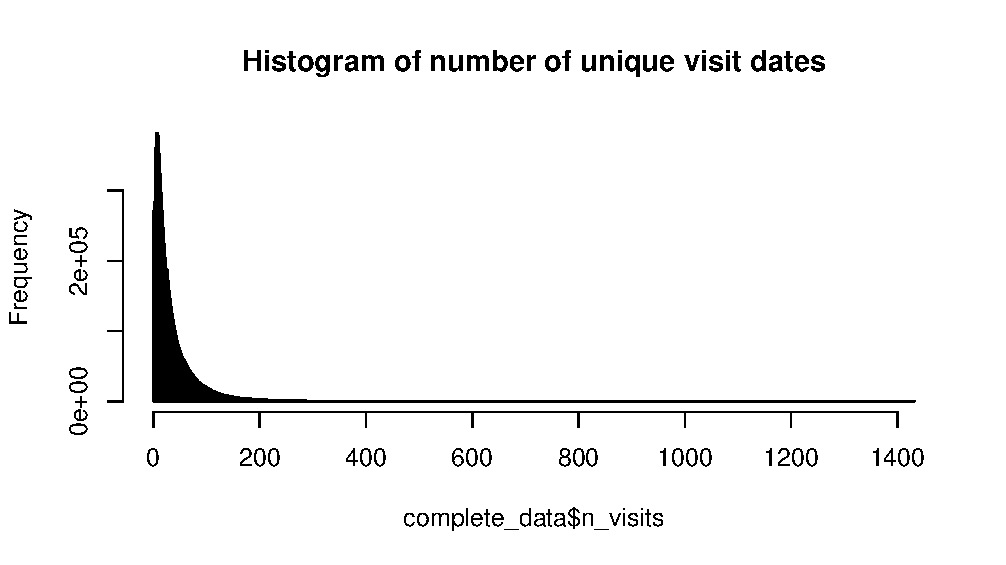
\includegraphics[width=.7\textwidth]{nvisits_hist.pdf}
\end{center}

The median control has 22 visits, while the median case has 33 visits.

Proportion of observed Charlson scores plotted against number of visits, separating controls (black) and cases (red):

\begin{center}
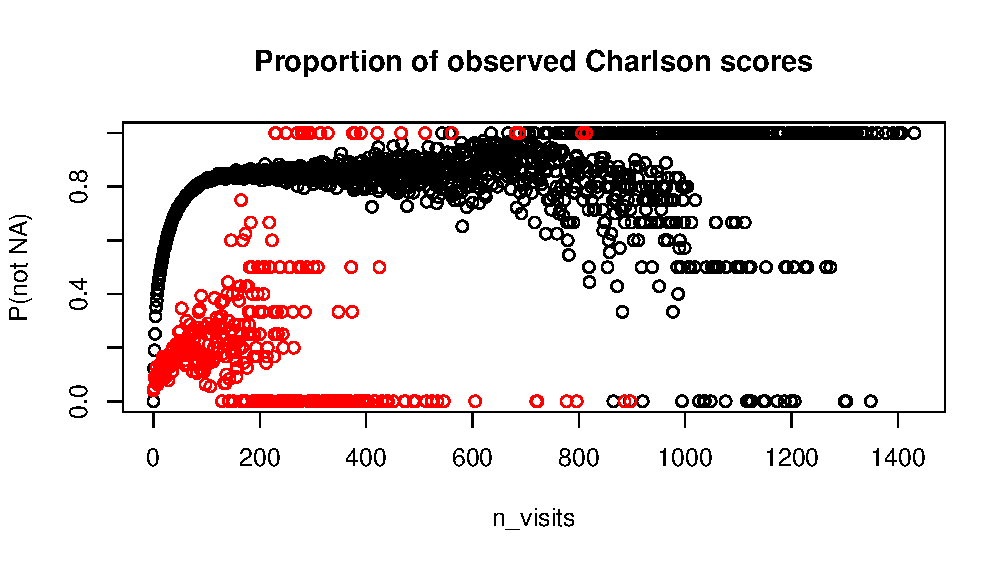
\includegraphics[width=.6\textwidth]{nvisits_scatter.pdf}
\end{center}

The same plot restricted to $\leq 200$ visits, where sample sizes are reasonably high (cases have a mean of 55 patients at each level of n\_visits):

\begin{center}
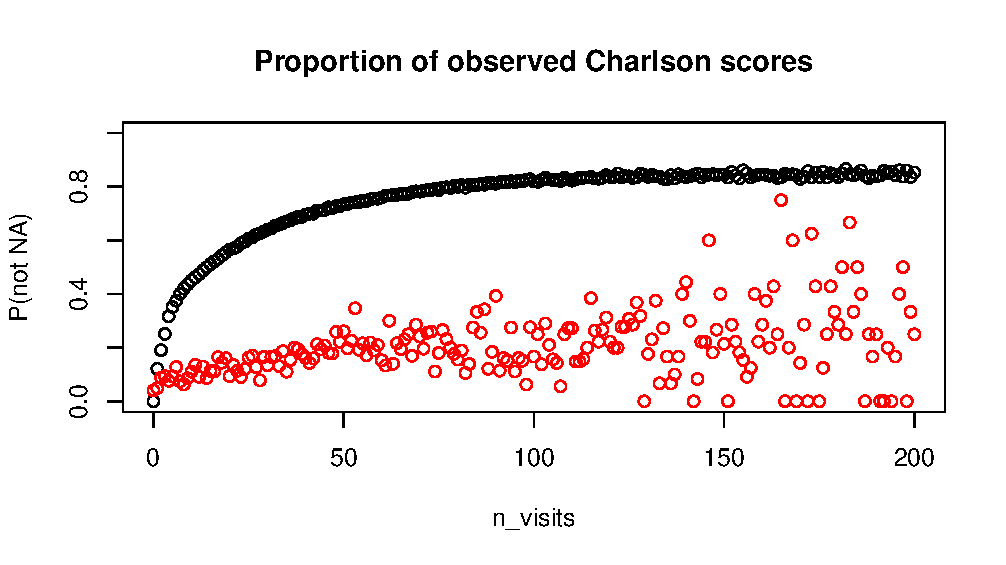
\includegraphics[width=.6\textwidth]{nvisits_scatter200.pdf}
\end{center}

Proportion of patient with COPD=1, plotted against number of visits, separating controls (black) and cases (red):

\begin{center}
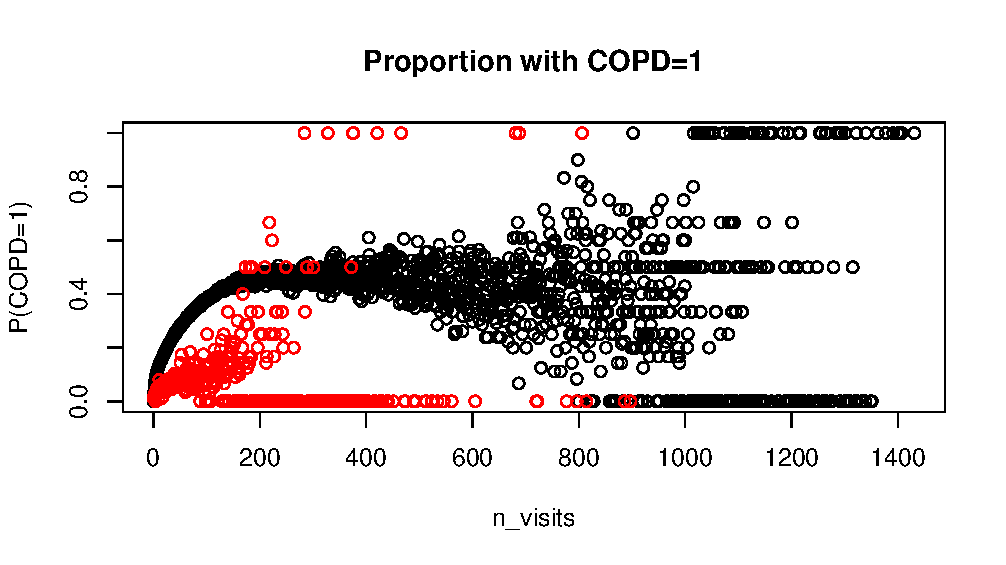
\includegraphics[width=.6\textwidth]{nvisits_scatterCOPD.pdf}
\end{center}

The same plot restricted to $\leq 200$ visits. The blue line is a parametric estimate of \\ $\mathbb{P}(\text{COPD}=1 | \text{n\_visits})$ based on the geometric model above fit to both cases and controls.

\begin{center}
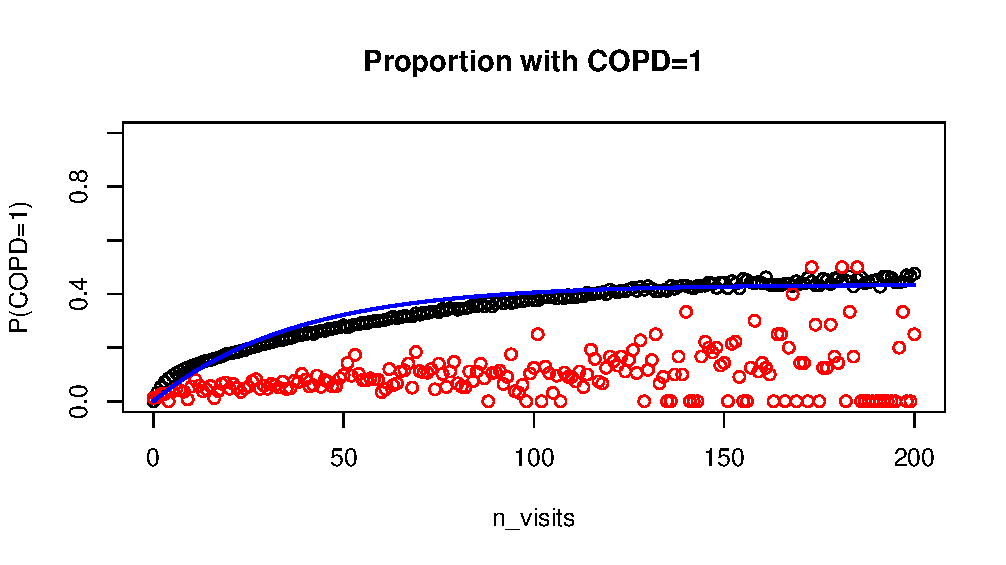
\includegraphics[width=.6\textwidth]{nvisits_scatterCOPD200.pdf}
\end{center}

\section*{Sample imbalance}

The full data is highly imbalanced, about 11,000 cases to over 6.6 million controls.

AUC's should be robust to this imbalance, but other evaluation metrics (decision curve analysis) may not be.

Proposed approaches are to either upweight the cases (weight parameter in xgboost), or to implement batched training which samples only a small set of controls to grow each tree(s).

\section*{Model evaluation/interpretation}

Currently, models are evaluated based on out-of-sample AUC, on 2 test sets of new observations, one with missing values (which are imputed the same way as the training data), and another with (mostly) observed records which are not imputed.

Akbar suggested another evaluation approach 'decision curve analysis', see 2 references to papers by Vickers (saved on gitlab).

The current esophogeal risk score for comparison is the Kunzmann score (see paper on Gitlab) which is a logistic regression model, and achieves an AUC of about 0.800.

There is a helper function 'xgb\_pdp' in utils\_xgb which produces marginal partial dependence plots for different predictors.

\section*{Meetings/updates}

Weekly updates/results are added to the file 'peter\_hosea\_updates.tex', the pdf is updated periodically on a HOSEA Dropbox folder (Maria can provide access).

%\bibliography{mybib}

\end{document}
